% !TEX root = main.tex
\subsection{Ceph Architecture}
\label{ceph-arch}

Ceph is one of many competing distributed storage systems. However, in the \ac{HPC} space, Ceph has not seen as much adoption as other \acs{HPC}-specialized file systems such as Lustre or BeeGFS. In the latest IO500 rankings at the time of writing~\cite{io500-full-list}, Ceph appears in 11 entries. These results are also not particularly high-ranking, in part due to the small number of nodes relative to the other systems. Therefore, how widely deployed Ceph is in production \ac{HPC} clusters is difficult to determine. At the time of writing, Ceph hard disk and \ac{SSD}-backed storage nodes are deployed at the \ac{GWDG} \ac{HPC} centers, which also provided access to the compute nodes used for this thesis.

In contrast to these more established \ac{HPC} file systems, Ceph is not designed around a specific field or use case. Rather, it is marketed as a flexible and reliable distributed storage system geared towards a large variety of use cases, from businesses to academic institutions~\cite{ceph-use-cases} through standard Ceph installations, as well as application-specific deployments using tools such as Rook on Kubernetes~\cite{rook-doc-home}.

To that end, Ceph provides a wide variety of storage types, including block devices, object storage, as well as a traditional file system interface. Fundamentally, Ceph is a software-defined object storage system designed to operate on a wide range of hardware, including commodity hardware. While storage systems such as Lustre require specific hardware configurations in order to achieve high availability and performance, Ceph is rather lenient in its hardware requirements, relying mostly on software to achieve the same goals.

% Ceph stands out as a versatile storage system due to its flexibility in
% implementation and usage. Its minimum requirements allow it to run on commodity
% hardware, which can make it easier for system administrators to get started with
% limited resources, such as those in small businesses. On the other hand, it is
% also designed to be scalable enough such that Ceph is a competitive file system
% in demanding applications such as \ac{HPC}. From a usage perspective, many
% storage systems in \ac{HPC} provide a pure file-system-based access method.
% Ceph, on the other hand, provides file system access as well, but it also
% provides its own optimized access method, RADOS, as well as object and block
% storage capabilities.

% Object storage can be easier from a data management perspective, especially when
% archival of large blobs of data are required. Block storage can be useful, for
% example, as a backing store for virtual machine disks.

% \subsection{Ceph Daemons}

% Ceph has several discrete components packaged into independent daemons, with
% each daemon performing a specific type of task. This modular design gives Ceph a
% high level of flexibility, allowing daemons to be placed on available hardware
% as needed. This includes the use of hardware with differing performance
% characteristics, which could potentially be optimized for performance or cost
% reasons.

\subsection{Ceph Daemons}

Ceph's storage architecture is not based on a single monolithic server application, but rather multiple daemons, each with specific responsibilities for the overall cluster. Because Ceph is designed to encompass several use cases, there are several types of daemons supported by it. Unless users require all of the functionality offered by Ceph, certain daemons can be enabled or disabled. The daemons required to enable Ceph's most basic functionality are shown in \Cref{tbl:ceph-required-daemons}. Note that these daemons only enable the use of Ceph's object storage service, but not its file system or other capabilities.

\begin{table}[htbp]
    \centering
    \begin{tabular}{|lll|}
        \hline
        \textbf{Daemon} & \textbf{Minimum} & \textbf{Recommended} \\
        \hline
        Monitor & 1       & 3 or 5        \\
        OSD     & 1       & 3+            \\
        Manager & 1       & 1 per monitor \\
        \hline
    \end{tabular}
    \caption[Required Ceph Daemons]{Daemons required for the functioning of Ceph's core \acs{RADOS} object storage service.}
    \label{tbl:ceph-required-daemons}
\end{table}

To access Ceph from different types of clients that may be unable to communicate directly using the \ac{RADOS} protocol, Ceph also allows for additional daemons and modules to be enabled. A list of the available modules and daemons are shown in~\cref{tbl:ceph-optional-daemons}.

\begin{table}[htbp]
    \centering
    \begin{tabular}{|llll|}
        \hline
        \textbf{Module/Daemon} & \textbf{Required for service} & \textbf{Minimum} & \textbf{Recommended} \\
        \hline
        MDS     & \acs{CephFS}                 & 1       & 2           \\
        RGW     & \acs{S3}/Swift Compatibility & 1       & -           \\
        NFS     & \acs{NFS}                    & 1       & -           \\
        iSCSI   & iSCSI                  & 1       & -           \\
        NVMeoF  & NVMeoF                 & 1       & -           \\  
        \hline
    \end{tabular}
    \caption[Additional Ceph Modules]{List of additional Ceph modules and daemons.}
    \label{tbl:ceph-optional-daemons}
\end{table}

A functional Ceph installation can be deployed on a single node, albeit with a limited amount of fault-tolerance. Ceph does not place a hard requirement on nodes having a certain number of daemons enabled, and it is the administrator's task to ensure that the system is configured such that the required level of redundancy is achieved.

The effect of this flexible design is that it is possible in Ceph to use heterogeneous nodes for storage--a feature that can be useful for clusters not designed to be a fixed size from the outset, but rather those that grow naturally with increasing or decreasing demands. In an \ac{HPC} scenario, one could start with a small cluster designed to fit current demands, and expand the cluster incrementally with new hardware as the amount of data stored on it or the number of users increases over time. From a procurement standpoint, this can spread capital expenditure over a longer period, but the benefits and drawbacks of this are out of the scope of this thesis.

\subsubsection{Monitors}

Monitors, also shortened in Ceph's administration utilities and documentation to ``mons'', are relatively simple daemons responsible for maintaining the consistent state of the cluster\footnote{\url{https://docs.ceph.com/en/latest/rados/configuration/mon-config-ref/\#monitor-config-reference}. Accessed 01.03.2026.}. Monitors communicate between each other and detect failures, and are responsible for the authentication of and providing cluster information to clients and other daemons. The monitors are not responsible for the vast majority of the data traffic on the system, which happens directly between clients and other Ceph daemons.

\subsubsection{Object Storage Daemons}

All Ceph storage services are built on top of the same underlying object storage protocol, known as \ac{RADOS}~\cite{ceph-discover}. Although Ceph supports multiple interfaces to access the data stored within it, including traditional hierarchical file storage, \ac{RADOS} is always the underlying layer at which data are ultimately stored. This protocol makes up Ceph's implementation of a highly-available object storage system.

\acp{OSD} are daemons responsible for directly interfacing with storage devices, forming the \ac{RADOS} backend. Data management tasks, such as object storage and some replication tasks, are performed by the \acs{OSD}'s communication with both its own attached storage device, as well as with other \acp{OSD} in the cluster. In a typical Ceph setup, disks are typically mapped to a single \ac{OSD}---if the storage medium is particularly fast, such as \ac{NVMe} flash storage, more \acp{OSD} per physical storage device may be desirable to extract the maximum available performance out of the device~\cite{ceph-blog-osd-per-disk}. 

The Ceph data resiliency concept is not generally achieved through redundancy built into individual \acp{OSD} through solutions such as \ac{RAID}. Rather, the distribution of data across multiple \acp{OSD} is performed through the use of an algorithm known as \ac{CRUSH}, which is described in \Cref{sec:ceph-crush}.

\subsubsection{\acs{CRUSH} Algorithm}
\label{sec:ceph-crush}

Having introduced \acp{OSD} as the basic storage units within Ceph, the
remaining problem is achieving redundancy when working under the assumption that
nodes are prone to failure~\cite[p. 307]{ceph-paper}. Ceph's solution to this
issue is fundamentally different relative to systems such as Lustre; whereas
Lustre backends often rely on the underlying hardware to be reliable~\cite{lustre-ha-wiki-zfs, lustre-ha-wiki}, using solutions such as \ac{RAID},
multi-pathing, and dedicated \acp{SAN}, among others, Ceph achieves its
reliability targets almost entirely through software solutions.

This design shifts a large amount of the complexity and cost of hardware-based
redundancy to, theoretically, an easier and more flexible solution to maintain.
This approach has the potential to reduce costs and efforts involved with both
the deployment of the cluster as well as changing the data layout. Putting these
considerations together lead to the development of \ac{CRUSH}, the system
responsible for the management of data replication and placement across
\acp{OSD} in Ceph clusters. As opposed to a traditional \ac{RAID}, individual
\acp{OSD} are discouraged from having redundancy on their own (e.g., running an
\ac{OSD} on top of a 2-disk
\ac{RAID})~\cite{rh-ceph-storage-raid}, delegating the task to \ac{CRUSH}. 

Fundamental to \acs{CRUSH}'s operation is the \ac{CRUSH} map~\cite{crush-paper}, which describes
the cluster topology and rules used for data distribution. Given this
information, clients can compute the storage location for a given object without
the need to exchange significant amounts of potentially fast-changing metadata.
The \ac{CRUSH} map represents the Ceph cluster as a hierarchy of buckets.
\acp{OSD} are grouped into these buckets, and the buckets are further grouped
into other buckets to form a logical hierarchy. The groups can be defined
flexibly to suit various topologies, although Ceph by default contains a few
predefined groups, such as the node and rack groups. Placement rules can then be
set on pools. Pools are logical partitions within a Ceph cluster, which contain
their own namespace---that is, identically-named objects from one pool are
isolated from each other---as well as the aforementioned placement rules.

\begin{figure}[h!]
    \centering
    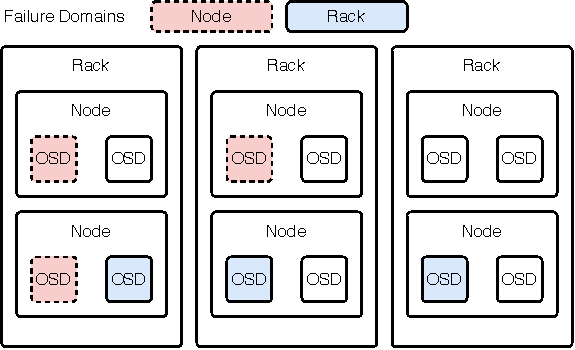
\includegraphics[width=0.5\linewidth]{assets/ceph/crush_failure_domains.pdf}
    \caption{CRUSH Failure Domains}
    \label{fig:crush-failure-domains}
\end{figure}

\Cref{fig:crush-failure-domains} demonstrates how this can be applied in
practice. For instance, for Ceph to protect against node failure resulting in
the loss of data, the placement rule's failure domain may be set at the node
level in the \ac{CRUSH} rule. In order to protect data against the failure of an
entire rack, the rule can be adapted accordingly and the placement is adjusted.
In this specific case, the object can withstand the loss of any two racks
without losing data. For \ac{HPC} specific use cases, it may be beneficial to
limit the replication in order to reduce latency. Placement rules may also
adjust the number of replicas (by default, this is three) or enable features
such as erasure coding.

Ceph also adds the \ac{PG} as an indirection layer for storage. Instead of
mapping an object directly to \acp{OSD}, the object is mapped to a \ac{PG}, and
the \acp{OSD} responsible for the \acp{PG} stores the \ac{PG} objects. This has
notable advantages over directly coupling objects to specific \acp{OSD}. The
main benefits are that recovery and balancing operations are greatly simplified.
Since object placement is tracked at the placement group level, determining the
data to be moved due to added or removed \acp{OSD} only requires knowing the
placement groups of the affected \ac{OSD}, of which there should typically not be more
than 100, according to Ceph recommended practices and defaults. The \ac{PG}
count can also remain static, even if the number of \acp{OSD} grows over time.

\subsubsection{\acs{CephFS}}

\ac{CephFS}---not to be confused with the Ceph storage system as a whole---is the file system support layer built on top of the existing Ceph \ac{RADOS} infrastructure. In effect, it acts as a translation layer between the hierarchical structure of a file system and the flat object storage that is Ceph's \ac{RADOS} layer. End users (in the context of this thesis, the users of the \ac{HPC} cluster) would simply see the file system without any changes needed to their workflows. In order to implement the file system, \ac{CephFS} relies on its \ac{MDS} daemons.

\subsubsection*{Metadata Servers}

\begin{figure}[htbp]
    \centering
    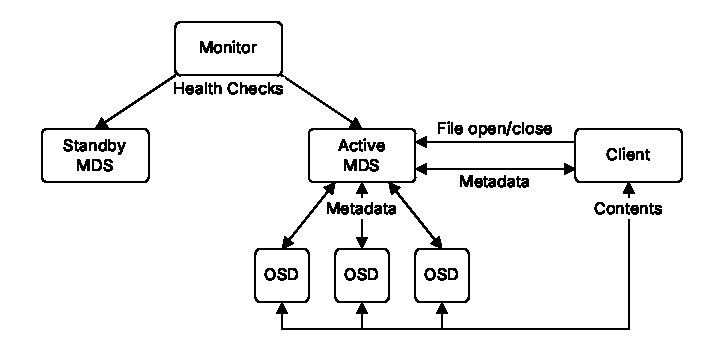
\includegraphics[width=0.9\textwidth]{assets/ceph/cephfs-mds-layout.pdf}
    \caption[CephFS Communication]
{Communication between Ceph \ac{MDS} daemons and clients as well as other Ceph
daemons in a CephFS setup. Clients request operations such as the
opening/closing of files from the \ac{MDS} and receive the appropriate metadata.
The contents of the files themselves are, however, written directly by the
client to the \acp{OSD}. Monitors perform health checking, instructing the
cluster to fail over to a standby \ac{MDS} in case the active \ac{MDS} fails.}
    \label{fig:cephfs-mds-layout}
\end{figure}

The \ac{MDS} is a core part of \acs{CephFS}. These daemons manage the state of the file system through synchronization with other \acs{MDS} daemons as well as acting as its source of truth for Ceph clients. However, for the actual file data itself, the client has access to the underlying \ac{RADOS} pool and can therefore communicate directly with \acp{OSD}, reducing the load on metadata servers. To achieve this, Ceph uses two separate pools for data and metadata, where the metadata may only be modified by \ac{MDS} daemons, and the data pool may be modified by Ceph clients directly. The metadata pool is also stored on top of \ac{RADOS}. The flow of operations is shown in \Cref{fig:cephfs-mds-layout}.

In order to improve metadata performance on slow pools, such as those backed by regular hard drives, the metadata pool may be on a separate storage class to that of the data pool. Since the metadata itself does not occupy as much space as the actual data, the metadata pool may be smaller than the bulk data pool. For instance, solid-state storage could be used. Common operations, such as a user listing their home directory, can then be served by this faster pool as well as the metadata cache of the \ac{MDS} itself.

\subsubsection*{Operating System Support}

On Linux, \ac{CephFS} supports three methods for accessing the Ceph file system: libcephfs, the \ac{FUSE} driver, and the kernel driver. The libcephfs library is a userspace library which allows applications to communicate directly with the Ceph cluster, i.e., with no mounting of the file system required. Of these three, the kernel driver is the most performant. However, it has the disadvantage of being bound to the kernel shipped with the distribution in use, unless a custom kernel is used.

\subsubsection{Comparison with Other File Systems}

Lustre shares some of the high-level design concepts with Ceph. Both cluster file systems are object stores at the lowest level, with a division of responsibilities between the management, storage, and metadata daemons, which can also be spread across multiple nodes~\cite[p.~308;pp.~6-9]{ceph-paper, lustre-manual}. However, the design philosophies of the two systems vary greatly.

Lustre, since its first full release, has historically been designed around achieving high performance and scalability for \ac{HPC} workloads\footnote{\url{https://lwn.net/Articles/63267/}. Dated 16.12.2003. Accessed 20.01.2026.}. In general, Lustre is not designed to provide redundancy for data, delegating this task to the lower level storage components, such as the underlying file system (e.g., ZFS) or a hardware \ac{RAID} controller. In this case, if a disk fails and is replaced, these lower-level components handle the necessary recovery steps. 

However, this does not provide failure tolerance in the case of node failure or other forms of hardware failure, such as cabling issues. In order for Lustre to be able to tolerate the failure of a single node, redundancy must be provided by external software. The recommended method for this is through the usage of Pacemaker and Corosync, which allows for failover of Lustre object storage servers~\cite{lustre-ha-wiki}, akin to a Ceph \ac{OSD} in terms of functionality. Nodes responsible for a specific \ac{OST} must both be connected to the storage (e.g., via an \ac{NVMeoF} connection to \acp{SSD}). This setup is shown in~\cref{fig:lustre-ha}. Without it, failure results in the data stored on that specific \ac{OST} becoming unreadable until the node is brought back up, and disk failure which cannot be corrected by the underlying storage system (e.g., 2-disk failure in a \acs{RAID}-5) results in the loss of all data on those disks.

\begin{figure}[htbp]
    \centering
    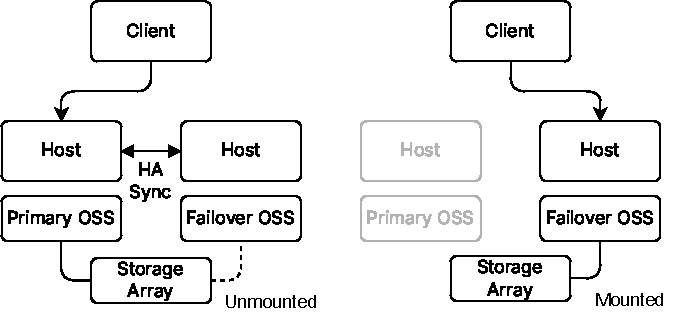
\includegraphics[width=0.75\linewidth]{assets/lustre/lustre_ha.pdf}
    \caption[Lustre \ac{HA} Concept]{High availability in the Lustre file system. Two nodes are connected to the same storage, with one node as the standby node. Upon failure of the primary node, the failover node takes over the task of serving the storage to clients. The Lustre architecture assumes that the underlying storage array is reliable, having a failover mode of its own.}
    \label{fig:lustre-ha}
\end{figure}

Versions of Lustre past 2.11.0, released in 2018\footnote{\url{https://www.lustre.org/lustre-2-11-0-released/}. Dated 03.04.2018. Accessed 20.01.2026.}, support a redundancy feature built into Lustre itself, known as \ac{FLR}. This feature allows for files to be replicated across multiple storage targets in a manner more similar to that of Ceph. However, the manual\footnote{\url{https://doc.lustre.org/lustre_manual.xhtml\#flr}. Accessed 20.01.2026.} describes this feature in more detail. Currently, this feature does not provide the strong guarantees that file systems such as ZFS or Ceph do---while writes are replicated to multiple object storage targets, they do not do so synchronously. A completed Lustre write on the client side with \ac{FLR}, therefore, does not guarantee that the desired replication level has been reached.

Overall, in its current revision, the underlying hardware must be highly reliable in order to be suitable for use within Lustre. However, possibly as a result of these assumptions, Lustre performs well as a \ac{HPC} file system~\cite{io500-full-list}. For instance, because no replication is used, the amount of network traffic can be reduced, increasing the amount of file \ac{I/O} operations possible within the bandwidth constraints.

\begin{figure}[htbp]
    \centering
    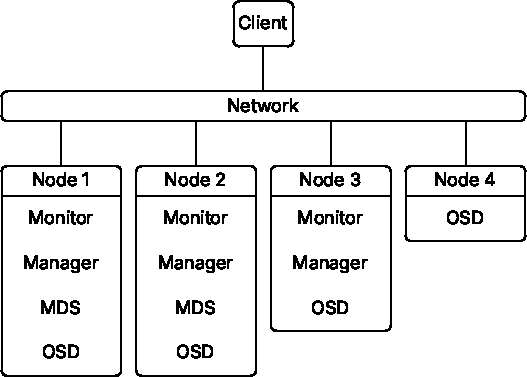
\includegraphics[width=0.5\linewidth]{assets/ceph/basic_ceph_cluster.pdf}
    \caption[Minimal Highly-Available Ceph Cluster]
    {
    The smallest highly-available Ceph cluster, containing the distribution of daemons necessary to allow for the continued functioning of the Ceph cluster after the failure of any one of the four nodes.
    }
    \label{fig:ceph-minimal-ha}
\end{figure}

Ceph, however, takes a much more conservative approach towards its expectations on hardware reliability~\cite{ceph-paper}, and is therefore much more flexible with its hardware requirements. While Lustre assumes the underlying hardware is reliable, Ceph assumes the hardware is unreliable and is therefore designed to handle failures on its own with its flexible \ac{CRUSH} algorithm, as detailed in~\cref{sec:ceph-crush}. This allows for the cluster to achieve its availability targets without highly-specialized hardware, potentially reducing costs. In~\cref{fig:ceph-minimal-ha}, a minimal highly-available cluster can be constructed with a small number of nodes, without \ac{RAID} on the \ac{OSD} backing storage. 

In summary, Lustre's approach to redundancy in the file system itself is explicitly opt-in, with none by default, while Ceph strongly discourages reducing redundancy. To opt out of redundancy in Ceph, it is not only necessary to enable the parameter mon\_allow\_pool\_size\_one, but to explicitly confirm intent when reducing pool sizes\footnote{\url{https://docs.ceph.com/en/latest/releases/pacific/}. Accessed 01.03.2026.}.



% Ceph, in this regard, is significantly more flexible with its hardware
% requirements. However, Lustre has historically performed well in
% \ac{HPC}~\cite{io500-full-list}, possibly as a result of these assumptions about
% the reliability of the underlying hardware. Network traffic, for instance, can
% be reduced significantly if no replication has to be performed.



% Due to the fact that Ceph is built with the presumption that nodes can and will
% fail, it performs its own health checks and maintains the redundancy level
% required by the user without the need for specific hardware or external
% software. This means, e.g., that instead of setting up a RAID-5 with 4 disks,
% the system administrator can instead assign one disk to one \ac{OSD} directly,
% and the required level of redundancy will be handled by Ceph according to the
% requirements (e.g., replica 3). This allows for the cluster to be highly
% available without requiring special hardware, which could potentially lower
% costs and increase reliability.


